\documentclass[12pt]{article}
%%% DOCUMENT FORMATTING %%%
\usepackage[margin=1in]{geometry}
\usepackage{enumitem}
\setlength{\parindent}{0pt}
\newcommand{\disp}{\displaystyle}

%%% HEADER %%%
\usepackage{fancyhdr}
\pagestyle{fancy}
\fancyhf{}
\lhead{MATH 1060}
\rhead{Vagnozzi}
\cfoot{\thepage}

%%% MATH NOTATION & SYMBOLS %%%
\usepackage{amssymb}
\usepackage{amsmath}
\newcommand{\R}{\mathbb{R}}
\newcommand{\N}{\mathbb{N}}
\newcommand{\Z}{\mathbb{Z}}
\newcommand{\lp}{\left(}
\newcommand{\rp}{\right)}
\newcommand{\ls}{\left[}
\newcommand{\rs}{\right]}
\newcommand{\lb}{\left\{}
\newcommand{\rb}{\right\}}
\newcommand{\arccot}{\text{arccot}}
\newcommand{\arccsc}{\text{arccsc}}
\newcommand{\arcsec}{\text{arcsec}} 

%%% TABLES %%%
\usepackage{colortbl}

%%% GRAPHS %%%
\usepackage{tikz}
\usepackage{pgfplots}
\pgfplotsset{compat=1.15}
\usepgfplotslibrary{fillbetween}
\usetikzlibrary{angles,quotes}

%%% ENVIRONMENTS %%%
\newcommand{\Example}{\paragraph{\Writinghand \hspace{0.1mm} Example.}}
\newcommand{\ExampleCont}{\paragraph{\Writinghand \hspace{0.1mm} Example (continued).}}
\newcommand{\boxenv}[2]{
	\fbox{
	\begin{minipage}{0.97\textwidth}
	\vspace{2mm}	
	\paragraph{#1} #2
	\vspace{2mm}
	\end{minipage}
	}}

%%% FUN THINGS %%%
\newcommand*\tc[1]{\tikz[baseline=(char.base)]{
            \node[shape=circle,draw,inner sep=2pt] (char) {#1};}}
\usepackage{marvosym}

%%% MISC %%%
\usepackage{hyperref}


\setcounter{page}{161}

\begin{document}
\section*{5.1: Approximating the Area Under a Curve}

\boxenv{Learning Objectives.}{Upon successful completion of Section 5.1, you will be able to\dots
		
	\begin{itemize}[leftmargin=6mm]
		\item Approximate displacement using a specified number of subintervals of a velocity \\ function.
		\item Answer conceptual questions involving areas under curves.
		\item Illustrate, calculate, and compare left, right, and midpoint Riemann sums.
		\item Evaluate Riemann sums from tables.
		\item Express given sums in sigma notation or evaluate expressions in sigma notation.
		\item Solve applications involving areas under curves.
	\end{itemize}
	\vspace{-4mm}
}

\vspace{5mm}

\subsection*{Sigma Notation}

The $\disp\Sigma$ (``sigma'') operator is used to express complicated or repetitive sums in compact form. For example, consider the following sum.

$$e^{-1}+2e^{-2}+3e^{-3}+\cdots +10e^{-10}=\sum_{i=1}^{10} ie^{-i}$$

\vspace{3mm}

The variable $i$ that appears beneath the $\disp\Sigma$ operator is an index, and the values below and above the $\disp\Sigma$ are the values at which this index begins and terminates, respectively. One way to interpret the sigma notation above is to say, ``Add all terms of the form $ie^{-i}$, where $i$ ranges from one to ten.'' Another variable besides $i$ may be used as the index ($j$, $k$, and $n$ are other popular choices).

\Example Express $1+4+9+16+25$ in sigma notation.

\vspace{20mm}

\Example Expand and evaluate the following sums.


\begin{itemize}
\item[\tc{1}] $\disp\sum_{i=1}^3\frac{i-1}{i}$
\end{itemize}

\newpage

\ExampleCont Expand and evaluate the following sums.

\begin{itemize}
	\item[\tc{2}] $\disp\sum_{i=1}^{4}(-1)^i\cos(i\pi)$
\end{itemize}

\vspace{15mm}

\paragraph{Properties of Sums.} The summation operation is \textit{linear}, meaning it has the following property.
$$\sum_{i=1}^{n}\big( af(i)\pm bg(i)\big)=a\sum_{i=1}^n f(i)\pm b\sum_{i=1}^n g(i),\text{ where }a,b\in\R$$

\vspace{3mm}

There are no results for division or multiplication within sums.

\vspace{5mm}

\paragraph{Special Sums.} The following special sums will often be useful when evaluating sums and will be critical for some of the examples in this chapter.

\vspace{5mm}

$\displaystyle\sum_{i=1}^{n}1=\underbrace{1+1+\cdots+1}_{n\text{ times}}=n$

\vspace{5mm}

$\displaystyle\sum_{i=1}^{n}c=c\sum_{i=1}^{n}1=cn$, where $c\in\R$

\vspace{5mm}

$\displaystyle\sum_{i=1}^{n}i=1+2+3+\cdots+n=\frac{n(n+1)}{2}=\frac{n^2+n}{2}$

\vspace{5mm}

$\displaystyle\sum_{i=1}^{n}i^2=1^2+2^2+3^2+\cdots+n^2=\frac{n(n+1)(2n+1)}{6}=\frac{2n^3+3n^2+n}{6}$

\vspace{5mm}

$\displaystyle\sum_{i=1}^{n}i^3=\left(\frac{n(n+1)}{2}\right)^2=\frac{n^4+2n^3+n^2}{4}$

\vspace{5mm}

$\displaystyle\sum_{i=1}^{n}i^4=\frac{n(n+1)(2n+1)(3n^2+3n-1)}{30}=\frac{6n^5+15n^4+10n^3-n}{30}$

\newpage

\subsection*{Area Under a Curve}

Consider the function $f(x)=x^2+1$ on the interval $[0,2]$, pictured  below. A key question of interest in calculus is: How can we measure the area between the graph of $f$ and the $x$-axis on the interval?

\begin{center}
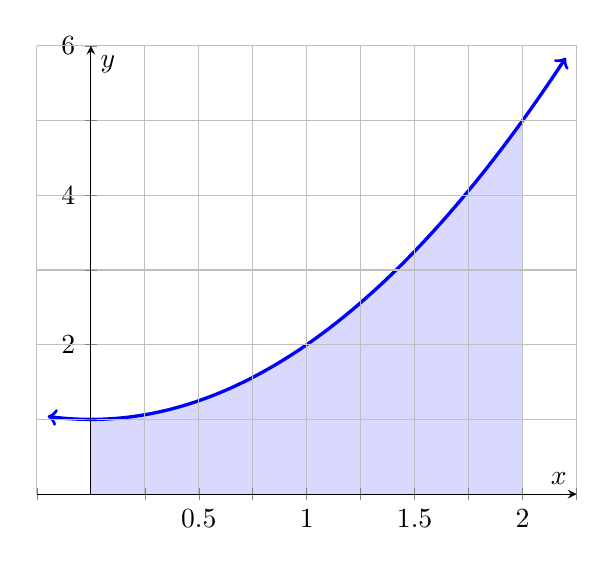
\begin{tikzpicture}
                \begin{axis}[grid=both, %minor tick num=1,
                	axis x line=middle,
			xtick={-.25,.25,.75,1.25,1.75,2.25},
			xticklabels={},
			ytick={0,1,3,5},
			yticklabels={},
			extra y ticks={2,4,6},
			extra x ticks={0.5,1,1.5,2},
                	xmax=2.25, xmin=-.25,
                	axis y line=center,
                	ymax=6, ymin=0,
	              	xlabel=$x$,ylabel=$y$, axis on top                    ]
                    \addplot[<->,name path=f,smooth,domain=-.2:2.2,color=blue,samples=100,very thick] {x^2+1};
		            \path[name path=axis] (axis cs:-1,0) -- (axis cs:4,0);
            
             \addplot+[blue!15] fill between[of=f and axis,soft clip={domain=0:2}];
                \end{axis}
            \end{tikzpicture}
            \end{center}
            
\vspace{3mm}

We will approximate such an area under a curve with rectangles.

\vspace{3mm}

\boxenv{Definition.}{A \textbf{partition} $\mathcal{P}$ of an interval $[a,b]$ is a finite ordered set $\lb x_i \rb$ such that $a=x_0<x_1<\cdots <x_k=b$. Each $\ls x_{i-1},x_i\rs$ is called a \textbf{subinterval} of $[a,b]$.}

\vspace{5mm}

Each interval $[a,b]$ has an infinite number of possible partitions. We let $\big|\mathcal{P}\big|$ denote the number of points in $\mathcal{P}$. For instance, $\mathcal{P}=\lb 0, 1, 2\rb$ is a partition of $[0,2]$ and $\big|\mathcal{P}\big|=3$.

\vspace{5mm}

\boxenv{Definition.}{A partition is called \textbf{uniform} if the distance between consecutive points is constant. This distance is called $\Delta x$ and is calculated by $\frac{b-a}{n}$ where $n=\big|\mathcal{P}\big|-1$.}

\vspace{5mm}

We will only consider uniform partitions. For a uniform partition $\mathcal{P}$ on $[a,b]$\dots
\begin{itemize}
	\item $n=\mathcal{P}-1$ is the number of subintervals for the partition.
	\item For each subinterval, we can create a rectangle with width $\Delta x=\disp\frac{b-a}{n}$.
	\item The sum of the areas of these rectangles yields our area approximation.
	
	\vspace{20mm}
\end{itemize}

\newpage

\Example Consider the uniform partition $\mathcal{P}_1=\lb 0,1,2\rb$ of $[0,2]$. Because $\big|\mathcal{P}_1\big|=3$, this partition gives two subintervals: $[0,1]$ and $[1,2]$. Let's approximate the area under the curve $f(x)=x^2+1$.

\vspace{5mm}

First, we will use \textbf{right-hand rectangles}.

\vspace{3mm}

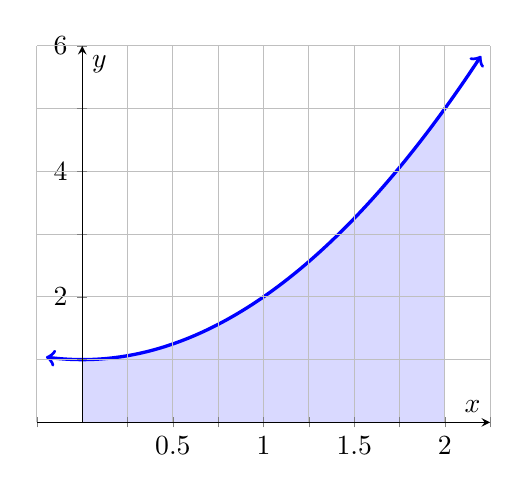
\begin{tikzpicture}[scale=0.84]
                \begin{axis}[grid=both, %minor tick num=1,
                	axis x line=middle,
			xtick={-.25,.25,.75,1.25,1.75,2.25},
			xticklabels={},
			ytick={0,1,3,5},
			yticklabels={},
			extra y ticks={2,4,6},
			extra x ticks={0.5,1,1.5,2},
                	xmax=2.25, xmin=-.25,
                	axis y line=center,
                	ymax=6, ymin=0,
	              	xlabel=$x$,ylabel=$y$, axis on top                    ]
                    \addplot[<->,name path=f,smooth,domain=-.2:2.2,color=blue,samples=100,very thick] {x^2+1};
		            \path[name path=axis] (axis cs:-1,0) -- (axis cs:4,0);
            
             \addplot+[blue!15] fill between[of=f and axis,soft clip={domain=0:2}];
                \end{axis}
            \end{tikzpicture}
            
            \vspace{5mm}

Now we will use \textbf{left-hand rectangles}.

\vspace{3mm}

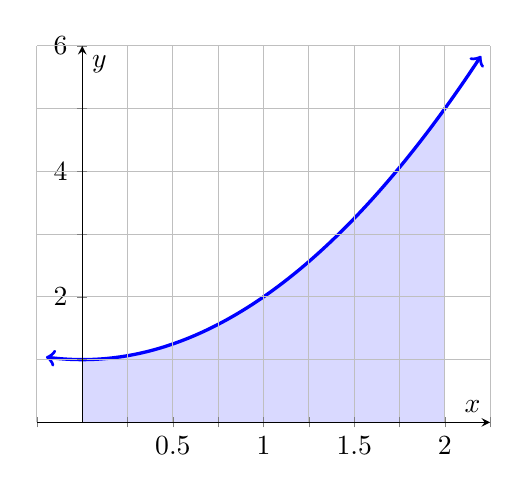
\begin{tikzpicture}[scale=0.84]
                \begin{axis}[grid=both, %minor tick num=1,
                	axis x line=middle,
			xtick={-.25,.25,.75,1.25,1.75,2.25},
			xticklabels={},
			ytick={0,1,3,5},
			yticklabels={},
			extra y ticks={2,4,6},
			extra x ticks={0.5,1,1.5,2},
                	xmax=2.25, xmin=-.25,
                	axis y line=center,
                	ymax=6, ymin=0,
	              	xlabel=$x$,ylabel=$y$, axis on top                    ]
                    \addplot[<->,name path=f,smooth,domain=-.2:2.2,color=blue,samples=100,very thick] {x^2+1};
		            \path[name path=axis] (axis cs:-1,0) -- (axis cs:4,0);
            
             \addplot+[blue!15] fill between[of=f and axis,soft clip={domain=0:2}];
                \end{axis}
            \end{tikzpicture}
            
            \vspace{5mm}

Lastly, we will use \textbf{midpoint rectangles}.

\vspace{3mm}

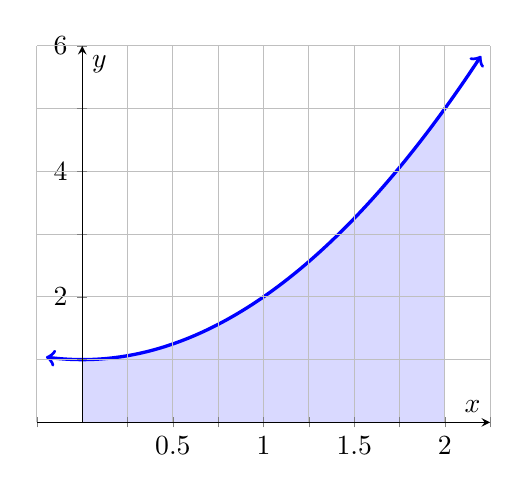
\begin{tikzpicture}[scale=0.84]
                \begin{axis}[grid=both, %minor tick num=1,
                	axis x line=middle,
			xtick={-.25,.25,.75,1.25,1.75,2.25},
			xticklabels={},
			ytick={0,1,3,5},
			yticklabels={},
			extra y ticks={2,4,6},
			extra x ticks={0.5,1,1.5,2},
                	xmax=2.25, xmin=-.25,
                	axis y line=center,
                	ymax=6, ymin=0,
	              	xlabel=$x$,ylabel=$y$, axis on top                    ]
                    \addplot[<->,name path=f,smooth,domain=-.2:2.2,color=blue,samples=100,very thick] {x^2+1};
		            \path[name path=axis] (axis cs:-1,0) -- (axis cs:4,0);
            
             \addplot+[blue!15] fill between[of=f and axis,soft clip={domain=0:2}];
                \end{axis}
            \end{tikzpicture}
            
\newpage

\ExampleCont Next, consider the uniform partition $\mathcal{P}_2=\lb 0, \frac{1}{2}, 1, \frac{3}{2}, 2\rb$ of $[0,2]$. Because $\big|\mathcal{P}_2\big|=5$, this partition gives four subintervals.

\vspace{5mm}

Approximate the area under $f$ using \textbf{right-hand rectangles}.

\vspace{3mm}

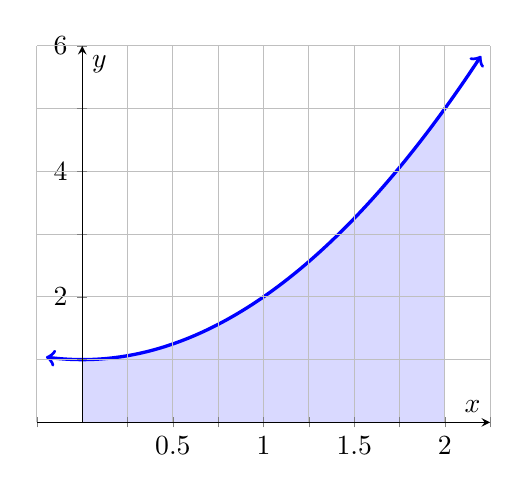
\begin{tikzpicture}[scale=0.84]
                \begin{axis}[grid=both, %minor tick num=1,
                	axis x line=middle,
			xtick={-.25,.25,.75,1.25,1.75,2.25},
			xticklabels={},
			ytick={0,1,3,5},
			yticklabels={},
			extra y ticks={2,4,6},
			extra x ticks={0.5,1,1.5,2},
                	xmax=2.25, xmin=-.25,
                	axis y line=center,
                	ymax=6, ymin=0,
	              	xlabel=$x$,ylabel=$y$, axis on top                    ]
                    \addplot[<->,name path=f,smooth,domain=-.2:2.2,color=blue,samples=100,very thick] {x^2+1};
		            \path[name path=axis] (axis cs:-1,0) -- (axis cs:4,0);
            
             \addplot+[blue!15] fill between[of=f and axis,soft clip={domain=0:2}];
                \end{axis}
            \end{tikzpicture}
            
            \vspace{5mm}

Approximate the area under $f$ using \textbf{left-hand rectangles}.

\vspace{3mm}

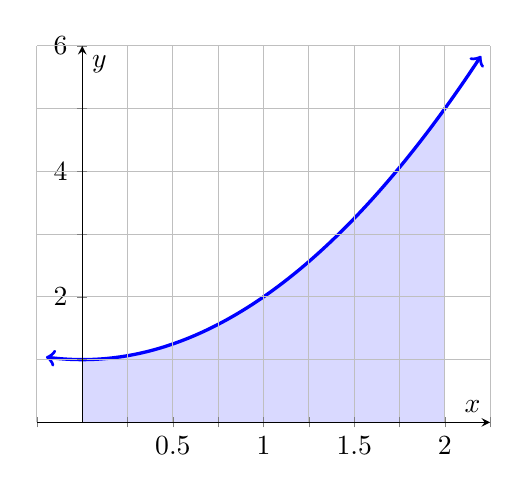
\begin{tikzpicture}[scale=0.84]
                \begin{axis}[grid=both, %minor tick num=1,
                	axis x line=middle,
			xtick={-.25,.25,.75,1.25,1.75,2.25},
			xticklabels={},
			ytick={0,1,3,5},
			yticklabels={},
			extra y ticks={2,4,6},
			extra x ticks={0.5,1,1.5,2},
                	xmax=2.25, xmin=-.25,
                	axis y line=center,
                	ymax=6, ymin=0,
	              	xlabel=$x$,ylabel=$y$, axis on top                    ]
                    \addplot[<->,name path=f,smooth,domain=-.2:2.2,color=blue,samples=100,very thick] {x^2+1};
		            \path[name path=axis] (axis cs:-1,0) -- (axis cs:4,0);
            
             \addplot+[blue!15] fill between[of=f and axis,soft clip={domain=0:2}];
                \end{axis}
            \end{tikzpicture}
            
            \vspace{5mm}

Approximate the area under $f$ using \textbf{midpoint rectangles}.

\vspace{3mm}

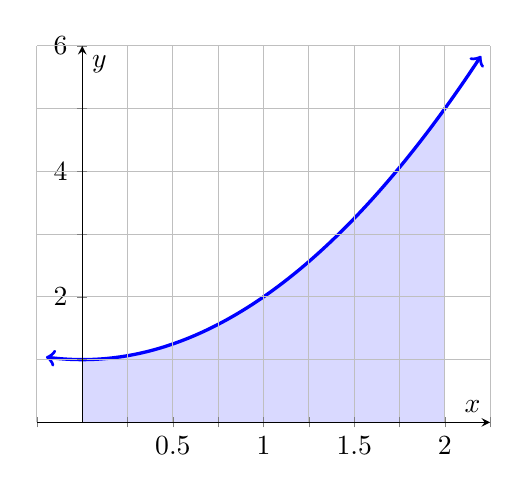
\begin{tikzpicture}[scale=0.84]
                \begin{axis}[grid=both, %minor tick num=1,
                	axis x line=middle,
			xtick={-.25,.25,.75,1.25,1.75,2.25},
			xticklabels={},
			ytick={0,1,3,5},
			yticklabels={},
			extra y ticks={2,4,6},
			extra x ticks={0.5,1,1.5,2},
                	xmax=2.25, xmin=-.25,
                	axis y line=center,
                	ymax=6, ymin=0,
	              	xlabel=$x$,ylabel=$y$, axis on top                    ]
                    \addplot[<->,name path=f,smooth,domain=-.2:2.2,color=blue,samples=100,very thick] {x^2+1};
		            \path[name path=axis] (axis cs:-1,0) -- (axis cs:4,0);
            
             \addplot+[blue!15] fill between[of=f and axis,soft clip={domain=0:2}];
                \end{axis}
            \end{tikzpicture}
            
\newpage

If we continue the example above with one more uniform partition, 
$$\mathcal{P}_3=\lb 0, \frac{1}{4},\frac{1}{2},\frac{3}{4},1,\frac{5}{4},\frac{3}{2},\frac{7}{4},2\rb,$$

we can see that $\big|\mathcal{P}_3\big|=9$, and thus $\mathcal{P}_3$ forms eight subintervals (i.e.\ eight rectangles) with 

$$\Delta x=\disp\frac{2-0}{8}=\frac{1}{4}.$$

\vspace{3mm}

Using eight rectangles yields the followings approximations.
\begin{itemize}
	\item Right-Hand Rectangles: $A\approx 5.1875$ units$^2$
	\item Left-Hand Rectangles: $A\approx 4.1875$ units$^2$
	\item Midpoint Rectangles: $A\approx 4.6563$ units$^2$
\end{itemize}

\vspace{5mm}

\subsection*{Riemann Sums}

What we have done in the preceding example is approximate the area between the curve $f$ and the $x$-axis using Riemann sums.

\vspace{3mm}

\boxenv{Definition.}{A sum of the following form is referred to as a \textbf{Riemann sum}.

$$\sum_{i=1}^n f(x_i^*)\Delta x_i$$

For a uniform partition, $\Delta x_i=\Delta x$.}

\vspace{5mm}

In general, the point $x_i^*$ may represent any point in the $i^{th}$ subinterval. If $x_i$ is\dots
\begin{itemize}
	\item a right-hand endpoint, this is referred to as a \textbf{right Riemann sum}.
	\item a left-hand endpoint, this is referred to as a \textbf{left Riemann sum}.
	\item a midpoint, this is referred to as a \textbf{midpoint Riemann sum}.
\end{itemize}

\newpage

\paragraph{Conclusions.} We can draw a few conclusions from our work thus far. Let $A$ represent the true area under $f(x)=x^2+1$ on $[0,2]$. Later, we will show that $A=\frac{14}{3}=4.\overline{6}$ units$^2$.
\begin{itemize}
	\item Note that we are only considering \textit{uniform} partitions (i.e.\ each interval/rectangle has the same width). This is not necessary, but it simplifies our discussion.
	\item Given a choice, the \textit{midpoint Riemann sum} typically gives the ``best'' approximation.
	\item As the number of rectangles $n$ gets very large, the right, left, and midpoint sums approach the true area, as demonstrated in the graph below.
	
	\begin{center}
		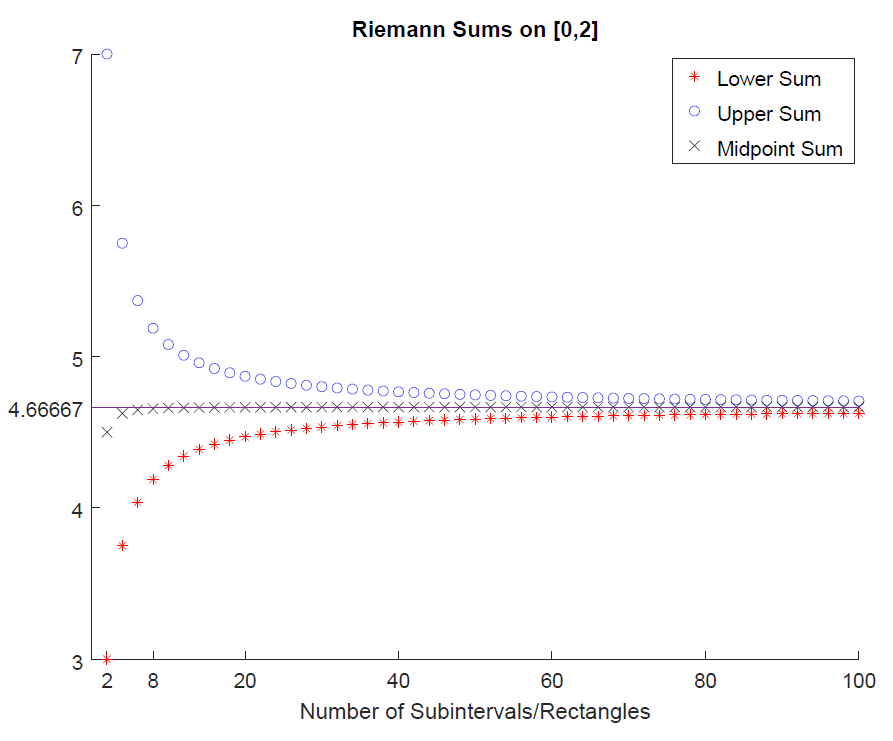
\includegraphics[scale=.9]{MATH_1060_Section_5-1_Riemann_Sums.PNG}
	\end{center}
\end{itemize}

What we are actually observing in the graph above is a \textit{limit}! As the number of approximating rectangles $n$ increases to infinity, we see that each sum converges to the true area $A=\frac{14}{3}$ units$^2$.

\newpage

The more rectangles we use in our Riemann sum, the better our approximation will be. This process can be rather tedious to do by hand. Fortunately, our understanding of limits will allow us to find this area exactly. First, let us consider a slightly more formalized definition of a Riemann sum.

\vspace{3mm}

\boxenv{Definition.}{Let $\mathcal{P}$ be an arbitrary partition of the interval $[a,b]$. A \textbf{Riemann sum} $S$ of $f$ over $[a,b]$ with partition $\mathcal{P}$ is defined by
$$S=\sum_{i=1}^n f(x_i^*)\Delta x_i\text{, where }x_i^*\in\ls x_{i-1},x_i\rs\text{ and }\Delta x_i=x_i-x_{i-1}.$$

Three common methods of choosing $x_i^*$ yield the left, right, and midpoint Riemann sums.}

\vspace{5mm}

If the partition $\mathcal{P}$ is uniform, any Riemann sum will converge to the \textbf{same value} as the number of points in the partition (i.e.\ the number of rectangles) goes to infinity.

\vspace{5mm}

\paragraph{General Case.} We define the \textbf{norm} of an arbitrary partition $\mathcal{P}$ of $[a,b]$ as

$$||\mathcal{P}||=\text{max}\lb\Delta x_1,\Delta x_2,\dots,\Delta x_n\rb,$$

\vspace{3mm}

where $\Delta x_i$ is the width of the $i^{th}$ subinterval. To obtain the true area, $A$, we let the width of the largest subinterval (rectangle) go to zero and find 

$$A=\lim_{||\mathcal{P}||\to 0}\sum_{i=1}^n f(x_i^*)\Delta x_i,$$

\vspace{3mm}

where $n=\mathcal{P}-1$ is the number of rectangles.

\vspace{5mm}

\paragraph{Uniform Case.} For a \textit{uniform} partition where $\Delta x_i=\Delta x=\disp\frac{b-a}{n}$, both $n\to\infty$ and $||\mathcal{P}||\to 0$ are equivalent. So, for a uniform partition, we have that

$$A=\lim_{||\mathcal{P}||\to 0}\sum_{i=1}^n f(x_i^*)\Delta x_i=\lim_{n\to \infty}\sum_{i=1}^n f(x_i^*)\Delta x,$$

\vspace{3mm}

provided the limit exists, where $x_i^*$ is any point in the $i^{th}$ subinterval.

\newpage

Algebraically, the right-hand endpoint is the easiest to work with. Thus, we formally define the area under a curve as \textit{the limit of a Riemann sum} in the following manner.

\vspace{3mm}

\boxenv{Area Under a Curve.}{Suppose that $f$ is a nonnegative, continuous function on $[a,b]$. The area, $A$, between the graph of $f$ and the $x$-axis on $[a,b]$ is found by calculating

$$A=\lim_{n\to\infty}\sum_{i=1}^n f(x_i^*)\Delta x,$$

where $\Delta x=\disp\frac{b-a}{n}$ and $x_i^*=a+i\Delta x$.}

\vspace{5mm}

Let's determine whether this limit functions in the way we would expect for finding the area under a curve in the following example.

\Example Using the definition for the area under a curve above, find the area of a triangle with base $b$ and height $h$.

\newpage 

\Example Now let's find the area under the graph of $f(x)=x^2+1$ on $[0,2]$. (This is the same area we approximated on pages 164--165 using a finite number of rectangles.)

\vspace{3mm}

\begin{flushright}
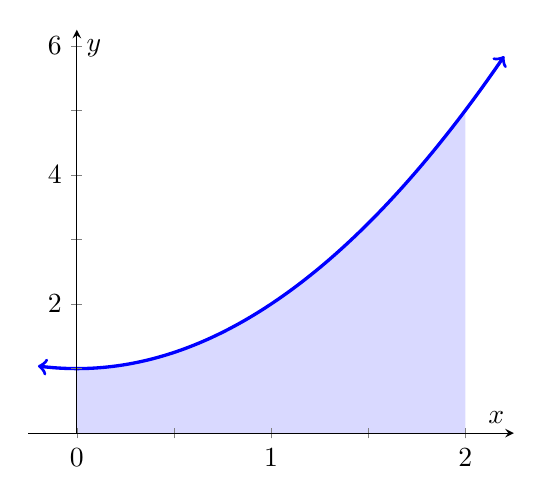
\begin{tikzpicture}[scale=.9]
                \begin{axis}[grid=none, %minor tick num=1,
                	axis x line=middle,
			xtick={-.5,.5,1,1.5,2,2.5},
			xticklabels={},
			ytick={0,1,3,5},
			yticklabels={},
			extra y ticks={2,4,6},
			extra x ticks={0,1,2},
                	xmax=2.25, xmin=-.25,
                	axis y line=center,
                	ymax=6.25, ymin=0,
	              	xlabel=$x$,ylabel=$y$, axis on top                    ]
                    \addplot[<->,name path=f,smooth,domain=-.2:2.2,color=blue,samples=100,very thick] {x^2+1};
		            \path[name path=axis] (axis cs:-1,0) -- (axis cs:4,0);
            
             \addplot+[blue!15] fill between[of=f and axis,soft clip={domain=0:2}];
                \end{axis}
            \end{tikzpicture}
\end{flushright}

\vspace{35mm}

\Example Find the area under the graph of $f(x)=x^3+2x$ on $\ls 0,\frac{3}{2}\rs$.

\begin{flushright}
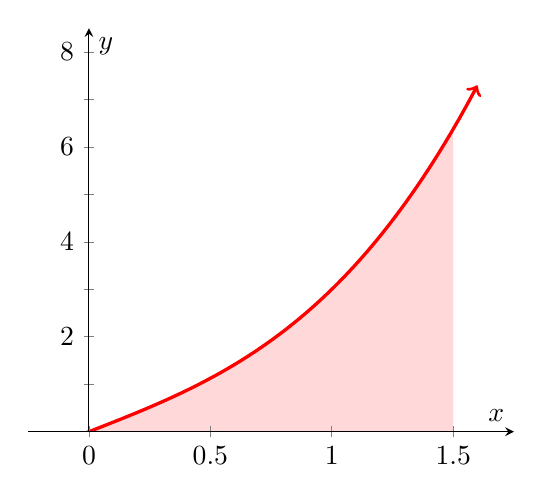
\begin{tikzpicture}[scale=.9]
                \begin{axis}[grid=none, %minor tick num=1,
                	axis x line=middle,
			xtick={-.5,.5,1,1.5,2},
			xticklabels={},
			ytick={0,1,3,5,7},
			yticklabels={},
			extra y ticks={2,4,6,8},
			extra x ticks={0,0.5,1,1.5},
                	xmax=1.75, xmin=-.25,
                	axis y line=center,
                	ymax=8.5, ymin=0,
	              	xlabel=$x$,ylabel=$y$, axis on top                    ]
                    \addplot[<->,name path=f,smooth,domain=-.2:1.6,color=red,samples=100,very thick] {x^3+2*x};
		            \path[name path=axis] (axis cs:-1,0) -- (axis cs:4,0);
            
             \addplot+[red!15] fill between[of=f and axis,soft clip={domain=0:1.5}];
                \end{axis}
            \end{tikzpicture}
\end{flushright}


\end{document}